% Section 1.1 Anatomy of Figures

\documentclass[nooutcomes]{ximera}
%\documentclass[space,handout,nooutcomes]{ximera}

% For preamble materials

\graphicspath{
  {./}
  {chapter1/}
  {chapter2/}
  {chapter4/}
  {math1/}
  {math2/}
}

\usepackage{pgf,tikz}
\usepackage{mathrsfs}
\usetikzlibrary{arrows}
\pgfplotsset{compat=1.16}


\newcommand{\N}{\mathbb N}
\newcommand{\W}{\mathbb W}
\newcommand{\C}{\mathbb C}
\newcommand{\Z}{\mathbb Z}
\newcommand{\Q}{\mathbb Q}
\newcommand{\R}{\mathbb R}




\title{Exploring Area}
\author{Brad Findell}
\begin{document}
\begin{abstract}
Short-answer problems about area and length. 
\end{abstract}
\maketitle

% Maybe add some problems that bring out the key principles about area

\begin{problem}
In the figures below, all vertices occur on dots, which are spaced by one cm, both vertically and horizontally.
\begin{image}
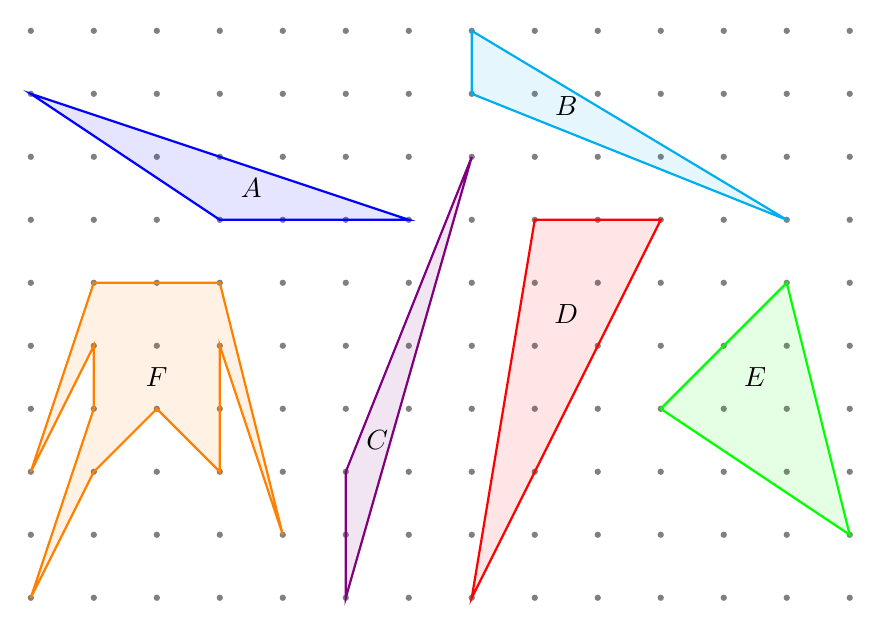
\begin{tikzpicture}[scale=0.8]
\foreach \x in {0,1,...,13} {
    \foreach \y in {0,1,...,9} {
        \fill[color=gray] (\x,\y) circle (0.05);
    }
 }
\draw[line width=0.8pt,color=blue,fill=blue,fill opacity=0.10] (3,6) -- (6,6) -- (0,8) -- cycle;
\draw (3.5,6.5) node {$A$};
\draw[line width=0.8pt,color=cyan,fill=cyan,fill opacity=0.10] (7.,8.) -- (7.,9.) -- (12.,6.) -- cycle;
\draw (8.5,7.8) node {$B$};
\draw[line width=0.8pt,color=violet,fill=violet,fill opacity=0.10] (5.,2.) -- (5.,0.) -- (7.,7.) -- cycle;
\draw (5.5,2.5) node {$C$};
\draw[line width=0.8pt,color=red,fill=red,fill opacity=0.10] (8.,6.) -- (7.,0.) -- (10.,6.) -- cycle;
\draw (8.5,4.5) node {$D$};
\draw[line width=0.8pt,color=green,fill=green,fill opacity=0.10] (10.,3.) -- (12.,5.) -- (13.,1.) -- cycle;
\draw (11.5,3.5) node {$E$};
\draw[line width=0.8pt,color=orange,fill=orange,fill opacity=0.10] (1.,2.) -- (0,0) -- (1,3) -- (1.,4.) -- (0.,2.) -- 
(1.,5.) -- (3,5) -- (4,1) -- (3,4) -- (3.,2.) -- (2,3) -- cycle;
\draw (2,3.5) node {$F$};
\end{tikzpicture}
\end{image}
Find the areas of the labeled regions: 
\begin{enumerate}
\item Area $A = \answer{3} \text{ cm}^2$.
\item Area $B = \answer{2.5} \text{ cm}^2$.
\item Area $C = \answer{2} \text{ cm}^2$.
\item Area $D = \answer{6} \text{ cm}^2$.
\item Area $E = \answer{5} \text{ cm}^2$.
\item Area $F = \answer{6.5} \text{ cm}^2$.
\end{enumerate}
\end{problem}

\newpage 

\begin{problem}
Finding areas and lengths.
\begin{image}
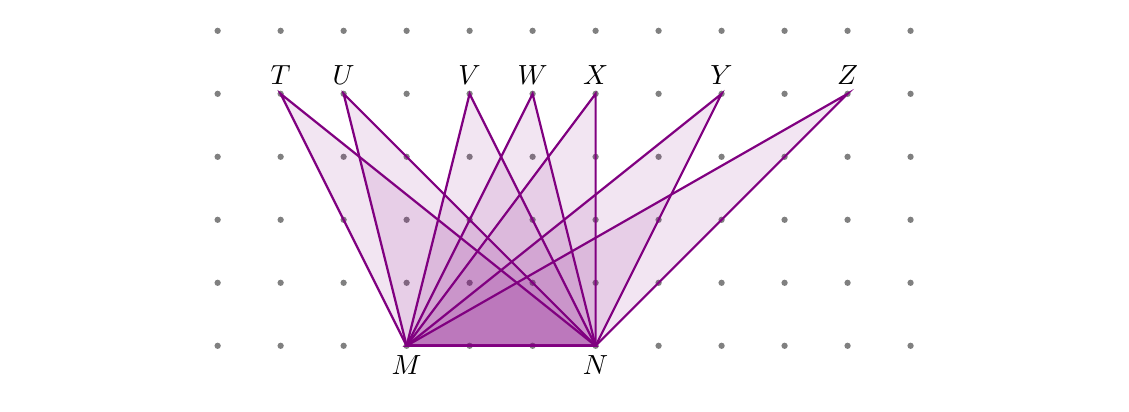
\begin{tikzpicture}[scale=0.8]
\foreach \x in {1,2,...,12} {
    \foreach \y in {0,1,...,5} {
        \fill[color=gray] (\x,\y) circle (0.05);
    }
 }
\draw[line width=0.8pt,color=violet,fill=violet,fill opacity=0.10] (4.,0.) -- (7.,0.) -- (2.,4.) -- cycle;
\draw[line width=0.8pt,color=violet,fill=violet,fill opacity=0.10] (4.,0.) -- (7.,0.) -- (3.,4.) -- cycle;
\draw[line width=0.8pt,color=violet,fill=violet,fill opacity=0.10] (4.,0.) -- (7.,0.) -- (5.,4.) -- cycle;
\draw[line width=0.8pt,color=violet,fill=violet,fill opacity=0.10] (4.,0.) -- (7.,0.) -- (6.,4.) -- cycle;
\draw[line width=0.8pt,color=violet,fill=violet,fill opacity=0.10] (4.,0.) -- (7.,0.) -- (7.,4.) -- cycle;
\draw[line width=0.8pt,color=violet,fill=violet,fill opacity=0.10] (4.,0.) -- (7.,0.) -- (9.,4.) -- cycle;
\draw[line width=0.8pt,color=violet,fill=violet,fill opacity=0.10] (4.,0.) -- (7.,0.) -- (11.,4.) -- cycle;
\draw (4.0,-0.3) node {$M$};
\draw (7.0,-0.3) node {$N$};
\draw (2.0,4.3) node {$T$};
\draw (3.0,4.3) node {$U$};
\draw (5.0,4.3) node {$V$};
\draw (6.0,4.3) node {$W$};
\draw (7.0,4.3) node {$X$};
\draw (9.0,4.3) node {$Y$};
\draw (11.0,4.3) node {$Z$};
\draw [color=white] (-2.,0.) circle (0.2pt);
\draw [color=white] (15.,0.) circle (0.2pt);
\end{tikzpicture}
\end{image}
Find the areas of triangles $TMN$, $UMN$, $VMN$, $WMN$, $XMN$, $YMN$, and $ZMN$. How do the areas compare? 
\begin{multipleChoice}
\choice{It is impossible to tell.}
\choice{They are all different.}
\choice[correct]{They are all the same.}
\choice{Some are the same and some are different.}
\end{multipleChoice}
\begin{problem}
This is true because they all have the same base of length $\answer{3}$ and equal heights of length $\answer{4}$. 
\end{problem}
\end{problem}

\newpage 

\begin{problem}
Finding areas and lengths.
\begin{image}
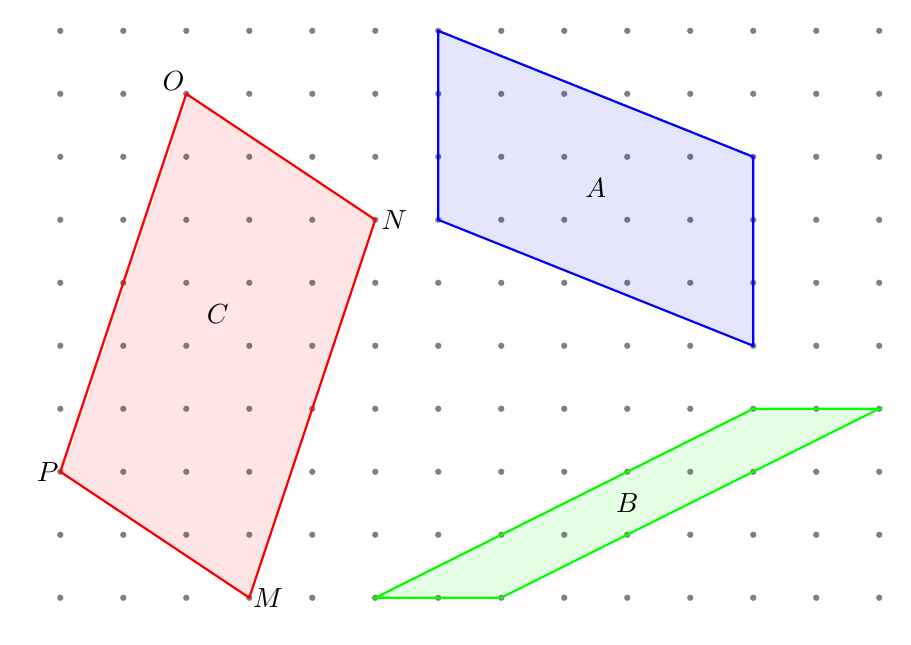
\begin{tikzpicture}[scale=0.8]
\foreach \x in {0,1,...,13} {
    \foreach \y in {0,1,...,9} {
        \fill[color=gray] (\x,\y) circle (0.05);
    }
 }
\draw[line width=0.8pt,color=blue,fill=blue,fill opacity=0.10] (6.,6.) -- (6.,9.) -- (11.,7.) -- (11.,4.) -- cycle;
\draw (8.5,6.5) node {$A$};
\draw[line width=0.8pt,color=green,fill=green,fill opacity=0.10] (5.,0.) -- (7.,0.) -- (13.,3.) -- (11.,3.) -- cycle;
\draw (9,1.5) node {$B$};
\draw[line width=0.8pt,color=red,fill=red,fill opacity=0.10] (0.,2.) -- (3.,0.) -- (5.,6.) -- (2.,8.) -- cycle;
\draw (2.5,4.5) node {$C$};
\draw (3.3,0) node {$M$};
\draw (5.3,6) node {$N$};
\draw (1.8,8.2) node {$O$};
\draw (-0.2,2) node {$P$};
\end{tikzpicture}
\end{image}
\begin{enumerate}
\item Using a vertical or horizontal base, in figure $A$, base = $\answer{3}$, height = $\answer{5}$ and area = $\answer{15}$.
\item Using a vertical or horizontal base, in figure $B$, base = $\answer{2}$, height = $\answer{3}$ and area = $\answer{6}$.
\item In figure $C$, none of the sides are horizontal or vertical, but area = $\answer{22}$.
\item In figure $C$, $MN = \answer{\sqrt{40}}$, so if $\overline{MN}$ is the base, the height must be $\answer{22/\sqrt{40}}$.
Note: To enter square roots, type \texttt{sqrt(5)} or use the math editor.  
\end{enumerate}
\end{problem}



\end{document}

